\documentclass[conference]{IEEEtran}
\IEEEoverridecommandlockouts
\usepackage{cite}
\usepackage{amsmath,amssymb,amsfonts}
\usepackage{graphicx}
\usepackage{booktabs}
\usepackage{textcomp}
\usepackage{xcolor}
\usepackage{url}
\renewcommand{\ttdefault}{cmtt} % Courier metrics are not installed in this TeX distribution
\graphicspath{{../figures/}}
\newcommand{\ResnetAcc}{71.1}
\newcommand{\ResnetBalAcc}{60.1}
\newcommand{\ResnetFone}{55.1}
\newcommand{\ResnetAuc}{0.918}
\newcommand{\ResnetParams}{23.5}
\newcommand{\ResnetGflops}{8.17}
\newcommand{\ResnetLat}{29.1}
\newcommand{\ResnetThr}{724}
\newcommand{\ResnetTrain}{20}
\newcommand{\ResnetEpoch}{85}
\newcommand{\ResnetVram}{1.8}
\newcommand{\ResnetBestEp}{12}
\newcommand{\ResnetEpNinetyfive}{6}
\newcommand{\ResnetEpRun}{12}
\newcommand{\ResnetFMEL}{58.5}
\newcommand{\ResnetFNV}{84.8}
\newcommand{\ResnetFBCC}{67.2}
\newcommand{\ResnetFAK}{43.8}
\newcommand{\ResnetFBKL}{51.5}
\newcommand{\ResnetFDF}{35.9}
\newcommand{\ResnetFVASC}{71.4}
\newcommand{\ResnetFSCC}{27.5}
\newcommand{\EffnetAcc}{73.8}
\newcommand{\EffnetBalAcc}{61.0}
\newcommand{\EffnetFone}{57.8}
\newcommand{\EffnetAuc}{0.906}
\newcommand{\EffnetParams}{4.0}
\newcommand{\EffnetGflops}{0.77}
\newcommand{\EffnetLat}{36.9}
\newcommand{\EffnetThr}{511}
\newcommand{\EffnetTrain}{14}
\newcommand{\EffnetEpoch}{61}
\newcommand{\EffnetVram}{1.5}
\newcommand{\EffnetBestEp}{8}
\newcommand{\EffnetEpNinetyfive}{5}
\newcommand{\EffnetEpRun}{12}
\newcommand{\EffnetFMEL}{61.7}
\newcommand{\EffnetFNV}{86.2}
\newcommand{\EffnetFBCC}{73.4}
\newcommand{\EffnetFAK}{36.2}
\newcommand{\EffnetFBKL}{57.3}
\newcommand{\EffnetFDF}{42.6}
\newcommand{\EffnetFVASC}{69.8}
\newcommand{\EffnetFSCC}{35.1}
\newcommand{\SwinAcc}{76.1}
\newcommand{\SwinBalAcc}{63.9}
\newcommand{\SwinFone}{64.1}
\newcommand{\SwinAuc}{0.900}
\newcommand{\SwinParams}{27.5}
\newcommand{\SwinGflops}{8.98}
\newcommand{\SwinLat}{71.2}
\newcommand{\SwinThr}{554}
\newcommand{\SwinTrain}{23}
\newcommand{\SwinEpoch}{105}
\newcommand{\SwinVram}{2.6}
\newcommand{\SwinBestEp}{8}
\newcommand{\SwinEpNinetyfive}{6}
\newcommand{\SwinEpRun}{12}
\newcommand{\SwinFMEL}{63.3}
\newcommand{\SwinFNV}{87.0}
\newcommand{\SwinFBCC}{74.6}
\newcommand{\SwinFAK}{44.8}
\newcommand{\SwinFBKL}{62.4}
\newcommand{\SwinFDF}{61.2}
\newcommand{\SwinFVASC}{80.9}
\newcommand{\SwinFSCC}{38.7}
\newcommand{\EnsAcc}{77.8}
\newcommand{\EnsBalAcc}{68.0}
\newcommand{\EnsFone}{66.5}
\newcommand{\EnsAuc}{0.942}
\newcommand{\EnsParams}{55.1}
\newcommand{\EnsGflops}{17.92}
\newcommand{\EnsLat}{137.1}
\newcommand{\EnsThr}{194}
\newcommand{\EnsFMEL}{65.4}
\newcommand{\EnsFNV}{88.3}
\newcommand{\EnsFBCC}{76.6}
\newcommand{\EnsFAK}{51.0}
\newcommand{\EnsFBKL}{63.7}
\newcommand{\EnsFDF}{64.2}
\newcommand{\EnsFVASC}{82.0}
\newcommand{\EnsFSCC}{40.4}
\newcommand{\BestModel}{Swin-T}
\newcommand{\BestFone}{64.1}
\newcommand{\Ntrain}{17,727}
\newcommand{\Nval}{3,844}
\newcommand{\Ntest}{3,760}
\newcommand{\Ntotal}{25,331}

\def\BibTeX{{\rm B\kern-.05em{\sc i\kern-.025em b}\kern-.08em T\kern-.1667em\lower.7ex\hbox{E}\kern-.125emX}}

\begin{document}

\title{CNNs versus Vision Transformers for Dermoscopic Skin-Lesion Classification:\\
A Controlled Comparison of ResNet-50, EfficientNet-B0 and Swin-T on ISIC 2019}

\author{\IEEEauthorblockN{José Alberto Martínez Navarro}
\IEEEauthorblockA{\textit{Universidad Panamericana (UPE)}\\
Aguascalientes, Mexico}
}

\maketitle

\begin{abstract}
Automated classification of dermoscopic images is a mature application of deep learning, yet
practitioners still face a practical question: should a clinical prototype be built on a
convolutional backbone or on a vision transformer, and at what computational price? We present a
controlled comparison of three ImageNet-pretrained architectures---ResNet-50, EfficientNet-B0 and
Swin-T---fine-tuned on the eight-class ISIC~2019 dataset (\Ntotal{} images) under a strictly
identical protocol: the same lesion-grouped stratified split, input resolution, augmentation,
optimiser, schedule, class-weighted loss and early-stopping rule. Beyond accuracy and macro-F1 we
report balanced accuracy, macro AUC, per-class F1, parameter count, FLOPs, peak training memory,
training time, epochs to convergence and inference latency on a single consumer GPU, and we
inspect the decision evidence of every model with Grad-CAM. On the held-out test split the best
single model, \BestModel{}, reaches \BestFone\% macro-F1, while a soft-voting ensemble of the
three backbones reaches \EnsFone\% macro-F1 and \EnsAuc{} macro AUC. The results show that the
accuracy gap between architecture families is small compared with their gap in cost, and that
the choice should be driven by the deployment budget rather than by the family label.
\end{abstract}

\begin{IEEEkeywords}
skin lesion classification, dermoscopy, ISIC 2019, convolutional neural networks, vision
transformers, transfer learning, Grad-CAM, computational cost
\end{IEEEkeywords}

\section{Introduction}
Skin cancer is among the most frequently diagnosed cancers worldwide and melanoma, its deadliest
form, is highly curable when detected early. Dermoscopy improves the diagnostic accuracy of
trained dermatologists, but access to specialists is uneven, which motivates computer-aided
diagnosis. Since Esteva~\textit{et al.}~\cite{esteva2017dermatologist} showed dermatologist-level
performance with a convolutional neural network (CNN), deep learning has become the standard
approach, and the International Skin Imaging Collaboration (ISIC) challenges
\cite{codella2018isic,tschandl2018ham10000,combalia2019bcn20000} have provided the public
benchmarks on which progress is measured.

Two developments make a fresh comparison worthwhile. First, vision transformers (ViT, Swin)
\cite{dosovitskiy2021vit,liu2021swin} now rival CNNs on natural images, and their suitability for
medical imaging, where datasets are small and class-imbalanced, is still debated
\cite{matsoukas2021transformers}. Second, in clinical and embedded settings the relevant question
is rarely ``which model is most accurate'' but ``which model is accurate \emph{enough} within a
given latency, memory and training budget''. Published results on ISIC are difficult to compare
because they differ in splits, resolutions, augmentation, ensembling and metadata usage
\cite{cassidy2022isic}.

This work therefore asks a narrow, controlled question: \emph{holding everything else fixed, how
do a classical CNN (ResNet-50), an efficiency-oriented CNN (EfficientNet-B0) and a hierarchical
vision transformer (Swin-T) compare on ISIC~2019 in accuracy, generalisation across classes,
computational cost and interpretability?} Our contributions are:
\begin{itemize}
  \item a reproducible, leakage-free experimental protocol (lesion-grouped stratified split,
        identical fine-tuning recipe) with open code;
  \item a multi-dimensional comparison covering accuracy, balanced accuracy, macro-F1, AUC,
        per-class behaviour, parameters, FLOPs, VRAM, training time, convergence speed and
        inference latency;
  \item a qualitative Grad-CAM analysis of what each architecture attends to, and a simple
        soft-voting ensemble that tests whether the families are complementary.
\end{itemize}

\section{Related Work}
\textbf{Datasets.} ISIC~2019 merges HAM10000~\cite{tschandl2018ham10000},
BCN20000~\cite{combalia2019bcn20000} and the MSK dataset into 25,331 dermoscopic images labelled
with eight diagnoses: melanoma (MEL), melanocytic nevus (NV), basal cell carcinoma (BCC), actinic
keratosis (AK), benign keratosis (BKL), dermatofibroma (DF), vascular lesion (VASC) and squamous
cell carcinoma (SCC). The distribution is strongly imbalanced (NV alone is about half of the
data) and several images may depict the same lesion, which can inflate scores if the split ignores
lesion identity~\cite{cassidy2022isic}.

\textbf{CNNs on ISIC.} The ISIC~2019 challenge was won by Gessert~\textit{et al.}
\cite{gessert2020isic2019} with a large ensemble of multi-resolution EfficientNets that also used
patient metadata, reaching a balanced accuracy of about 0.63 on the (harder, out-of-distribution)
official test set. Kassani and Kassani~\cite{kassani2019comparative} compared VGG, ResNet,
Xception and DenseNet~\cite{huang2017densenet} for melanoma detection and found ResNet-50 the most
accurate of the classical backbones. ImageNet pre-training
\cite{deng2009imagenet} is used almost universally; Raghu~\textit{et al.}
\cite{raghu2019transfusion} showed that, for medical images, its main benefit is faster
convergence rather than a large accuracy gain, and that lightweight networks can match large ones.

\textbf{Transformers in medical imaging.} The ViT~\cite{dosovitskiy2021vit} applies the
self-attention of~\cite{vaswani2017attention} to image patches; Swin~\cite{liu2021swin} restores
locality and a feature pyramid through shifted windows, which makes it a drop-in backbone for
dense tasks (e.g. TransUNet~\cite{chen2021transunet}). Matsoukas~\textit{et al.}
\cite{matsoukas2021transformers} found that, on small medical datasets, ViTs match CNNs only when
ImageNet-pretrained. Aladhadh~\textit{et al.}~\cite{aladhadh2022mvt} report competitive results of
a ViT on HAM10000. Most of these studies compare a single metric and rarely report the cost side;
our study fills that gap on ISIC~2019 with a strictly shared protocol.

\section{Methodology}
\subsection{Dataset and split}
We use the public ISIC~2019 training set (\Ntotal{} images, eight classes), the only part with
public labels. The official \texttt{lesion\_id} metadata is used to build a
\emph{lesion-grouped}, class-stratified split of \Ntrain{}/\Nval{}/\Ntest{} images
(train/validation/test, $\approx$70/15/15\%), so that no lesion appears in two splits
(Fig.~\ref{fig:dist}). The split is fixed (seed~42) and shared by all models.

\begin{figure}[t]
  \centering
  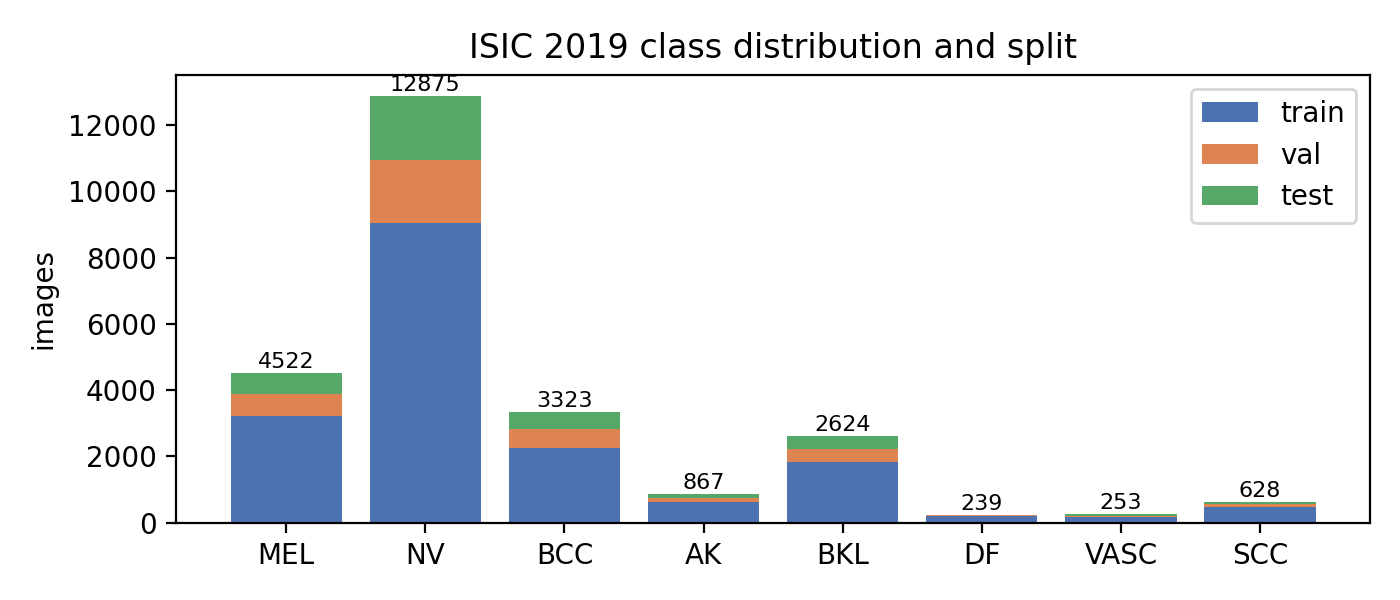
\includegraphics[width=\columnwidth]{class_dist.png}
  \caption{Class distribution of ISIC~2019 and the lesion-grouped train/validation/test split.}
  \label{fig:dist}
\end{figure}

\subsection{Pre-processing and augmentation}
Images are resized once to a shorter side of 256~px and centre-cropped to $256\times256$. During
training we apply random resized crops to $224\times224$ (scale 0.7--1.0), horizontal and vertical
flips, rotations up to $20^\circ$ and mild colour jitter; at evaluation the centre $224\times224$
crop is used. Pixels are normalised with ImageNet statistics. The same pipeline feeds every model.

\subsection{Models}
All backbones are taken from \texttt{timm}~\cite{wightman2019timm} with ImageNet-1k weights and a
new eight-way linear head, and are fine-tuned end to end:
\begin{itemize}
  \item \textbf{ResNet-50}~\cite{he2016resnet}: the reference residual CNN (\ResnetParams{}~M
        parameters, \ResnetGflops{}~GFLOPs).
  \item \textbf{EfficientNet-B0}~\cite{tan2019efficientnet}: a compound-scaled, mobile-oriented
        CNN (\EffnetParams{}~M, \EffnetGflops{}~GFLOPs).
  \item \textbf{Swin-T}~\cite{liu2021swin}: a hierarchical vision transformer with shifted-window
        attention (\SwinParams{}~M, \SwinGflops{}~GFLOPs), chosen over ViT-B because its cost is
        comparable to ResNet-50, which keeps the comparison fair.
\end{itemize}
As an exploratory variant we also evaluate a \textbf{soft-voting ensemble} that averages the
softmax outputs of the three fine-tuned models.

\subsection{Training protocol (identical for all models)}
Batch size 32, AdamW~\cite{loshchilov2019adamw} with learning rate $10^{-4}$ and weight decay
0.05, one warm-up epoch followed by cosine decay, at most 12 epochs with early stopping (patience
4) on validation macro-F1, gradient clipping at 1.0 and mixed-precision
training~\cite{micikevicius2018amp}. To counter class imbalance the cross-entropy loss is weighted
by the inverse square root of the class frequency and smoothed with $\epsilon=0.1$
\cite{muller2019labelsmoothing}. The checkpoint with the best validation macro-F1 is evaluated
once on the test split. All runs use a single NVIDIA RTX~4070 Laptop GPU (8~GB).

\subsection{Metrics}
\emph{Accuracy} and \emph{macro-F1} (required by the course), \emph{balanced accuracy} (the
official ISC~2019 metric), macro one-vs-rest \emph{AUC} and per-class F1 on the test split.
\emph{Cost}: trainable parameters, GFLOPs per image, peak training VRAM, mean epoch time, total
training time, the epoch of the best checkpoint and the number of epochs needed to reach 95\% of
the best validation F1 (convergence speed), and fp16 inference latency at batch~1 and throughput
at batch~32. \emph{Interpretability}: Grad-CAM~\cite{selvaraju2017gradcam} on the last
convolutional stage of the CNNs and on the last Swin block (tokens reshaped to a $7\times7$ map).

\section{Results}
\subsection{Overall performance and cost}
Table~\ref{tab:summary} summarises the test results. Training curves are shown in
Fig.~\ref{fig:curves} and the accuracy/cost trade-off in Fig.~\ref{fig:cost}.

\begin{table*}[t]
  \caption{Test-split results and computational cost under the shared protocol
  (fp16 latency on an RTX 4070 Laptop; ``Ep. 95\%'' = epochs to reach 95\% of the best validation macro-F1).}
  \label{tab:summary}
  \centering
  \resizebox{\textwidth}{!}{\begin{tabular}{llcccccccccccc}
\toprule
Model & Type & Acc. & Bal. Acc. & Macro-F1 & AUC & Params (M) & GFLOPs & Lat. (ms) & img/s & Train (min) & VRAM (MB) & Best ep. & Ep. 95\% \\
\midrule
ResNet-50 & CNN & 0.711 & 0.601 & 0.551 & 0.918 & 23.5 & 8.17 & 29.1 & 724 & 20.4 & 1807 & 12 & 6 \\
EfficientNet-B0 & CNN & 0.738 & 0.610 & 0.578 & 0.906 & 4.0 & 0.77 & 36.9 & 511 & 13.7 & 1500 & 8 & 5 \\
Swin-T & Transformer & 0.761 & 0.639 & 0.641 & 0.900 & 27.5 & 8.98 & 71.2 & 554 & 23.4 & 2667 & 8 & 6 \\
Ensemble (soft voting) & Hybrid & 0.778 & 0.680 & 0.665 & 0.942 & 55.1 & 17.92 & 137.1 & 194 & -- & -- & -- & -- \\
\bottomrule
\end{tabular}}
\end{table*}

\begin{figure*}[t]
  \centering
  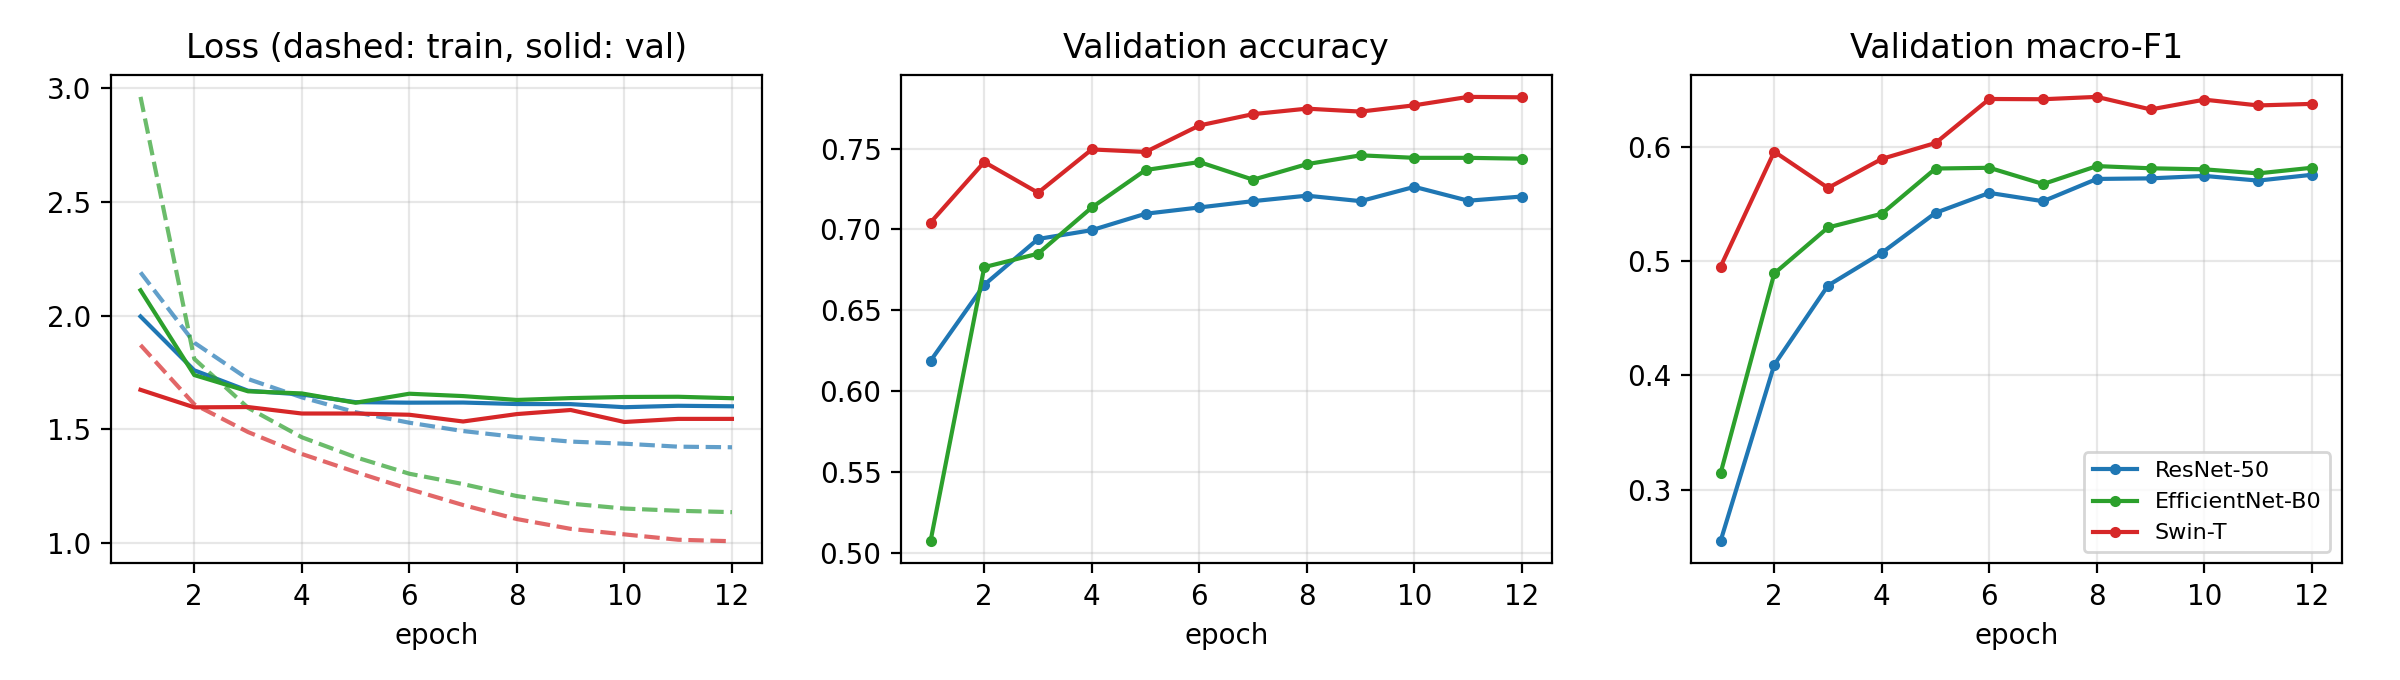
\includegraphics[width=\textwidth]{curves.png}
  \caption{Training/validation loss, validation accuracy and validation macro-F1 per epoch.}
  \label{fig:curves}
\end{figure*}

\begin{figure}[t]
  \centering
  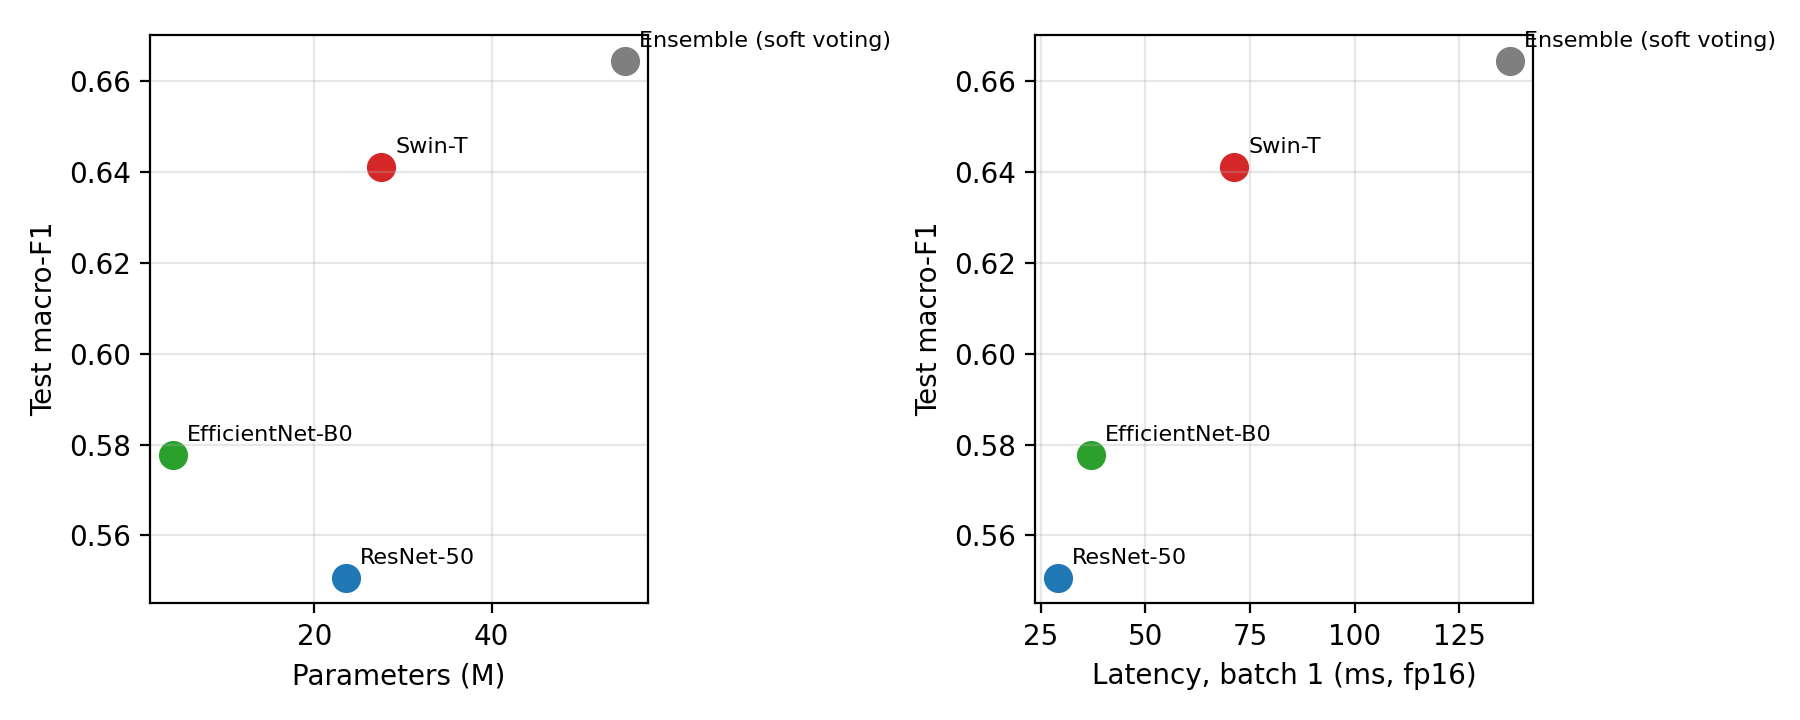
\includegraphics[width=\columnwidth]{acc_vs_cost.png}
  \caption{Test macro-F1 versus parameters (left) and batch-1 latency (right).}
  \label{fig:cost}
\end{figure}

\subsection{Per-class behaviour}
Table~\ref{tab:perclass} and Fig.~\ref{fig:perclass} report the per-class F1, and
Fig.~\ref{fig:cm} the confusion matrices.

\begin{table}[t]
  \caption{Per-class test F1.}
  \label{tab:perclass}
  \centering
  \resizebox{\columnwidth}{!}{\begin{tabular}{lcccccccc}
\toprule
Model & MEL & NV & BCC & AK & BKL & DF & VASC & SCC \\
\midrule
ResNet-50 & 0.58 & 0.85 & 0.67 & 0.44 & 0.51 & 0.36 & 0.71 & 0.28 \\
EfficientNet-B0 & 0.62 & 0.86 & 0.73 & 0.36 & 0.57 & 0.43 & 0.70 & 0.35 \\
Swin-T & 0.63 & 0.87 & 0.75 & 0.45 & 0.62 & 0.61 & 0.81 & 0.39 \\
Ensemble (soft voting) & 0.65 & 0.88 & 0.77 & 0.51 & 0.64 & 0.64 & 0.82 & 0.40 \\
\bottomrule
\end{tabular}}
\end{table}

\begin{figure}[t]
  \centering
  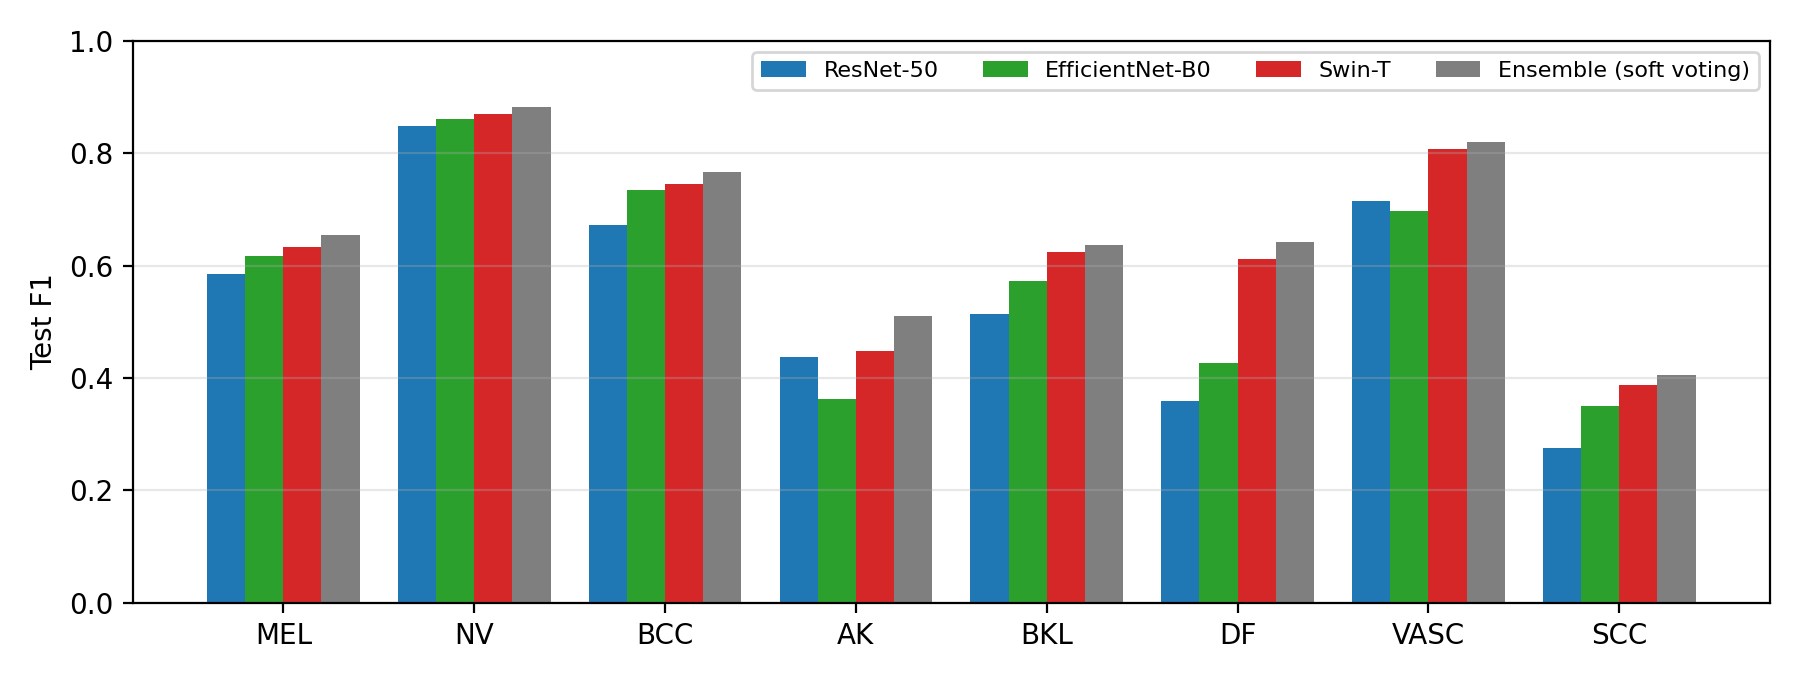
\includegraphics[width=\columnwidth]{per_class_f1.png}
  \caption{Per-class test F1 of each model.}
  \label{fig:perclass}
\end{figure}

\begin{figure*}[t]
  \centering
  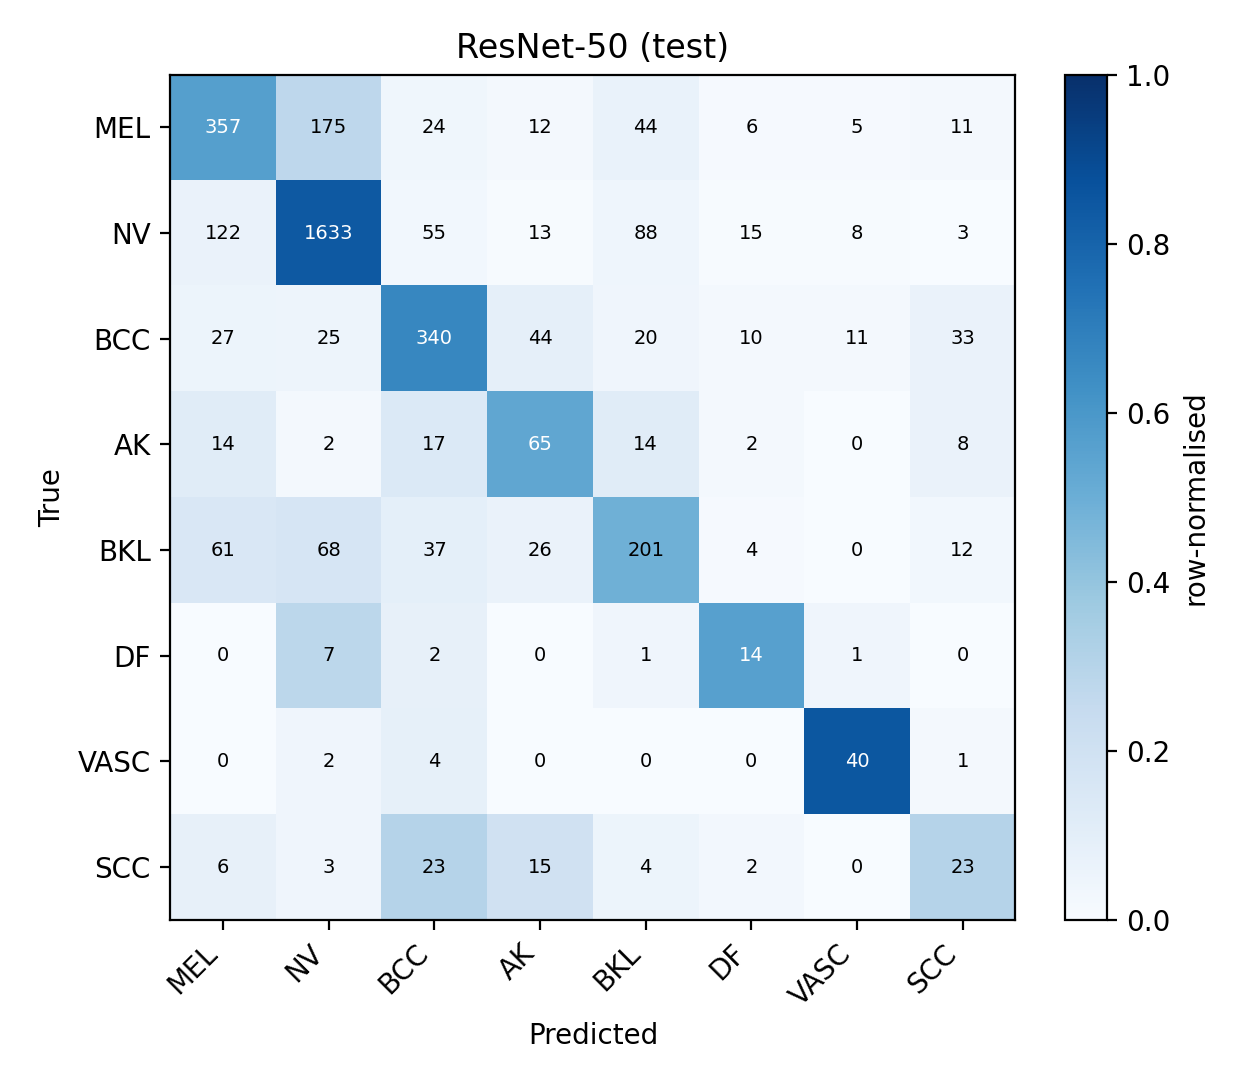
\includegraphics[width=0.32\textwidth]{cm_resnet50.png}
  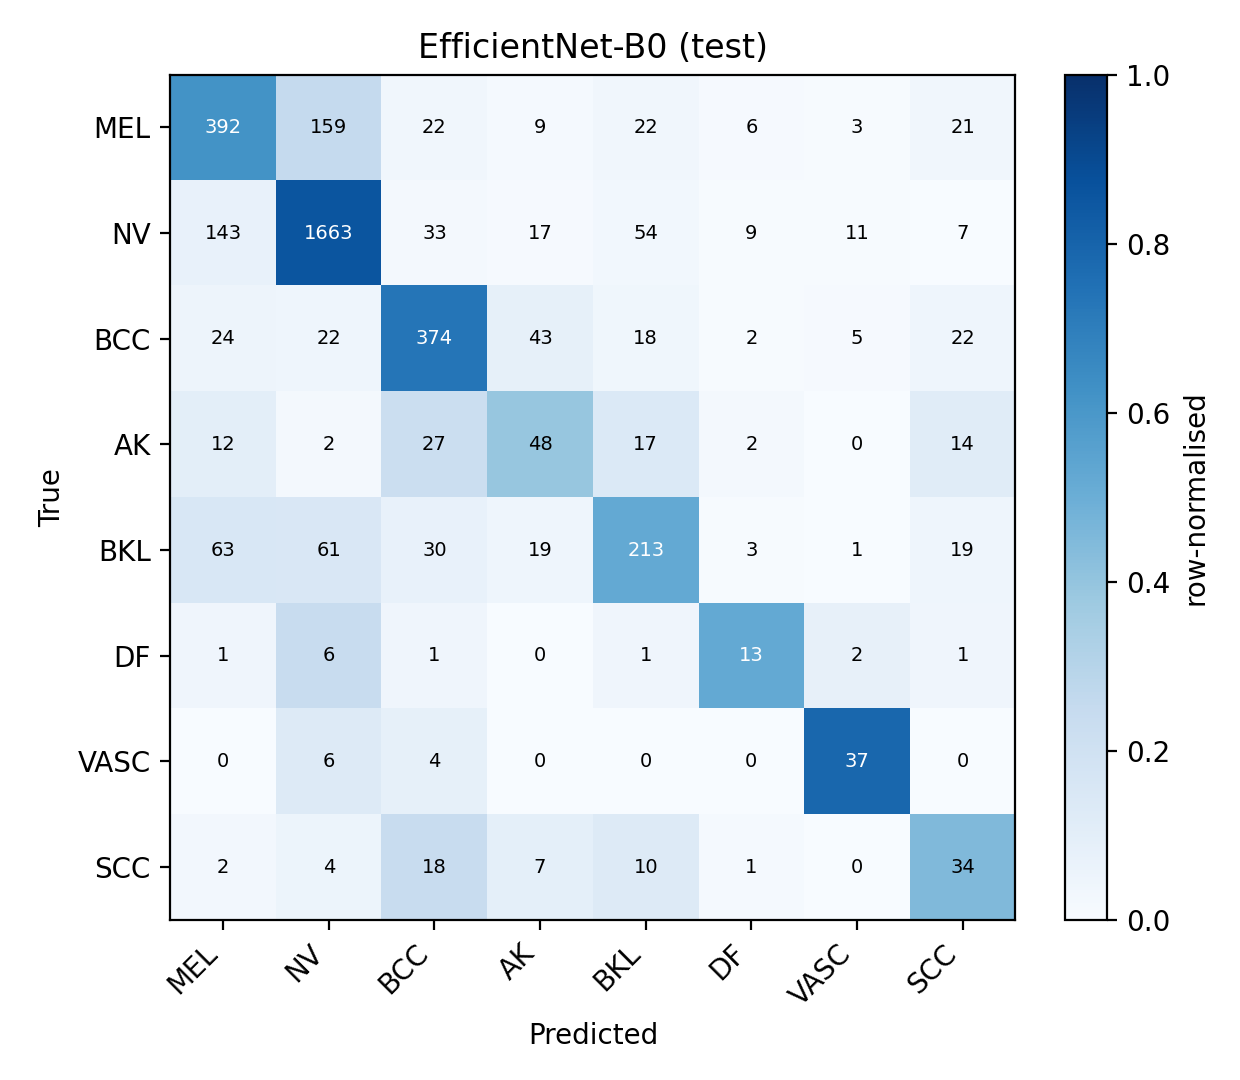
\includegraphics[width=0.32\textwidth]{cm_efficientnet_b0.png}
  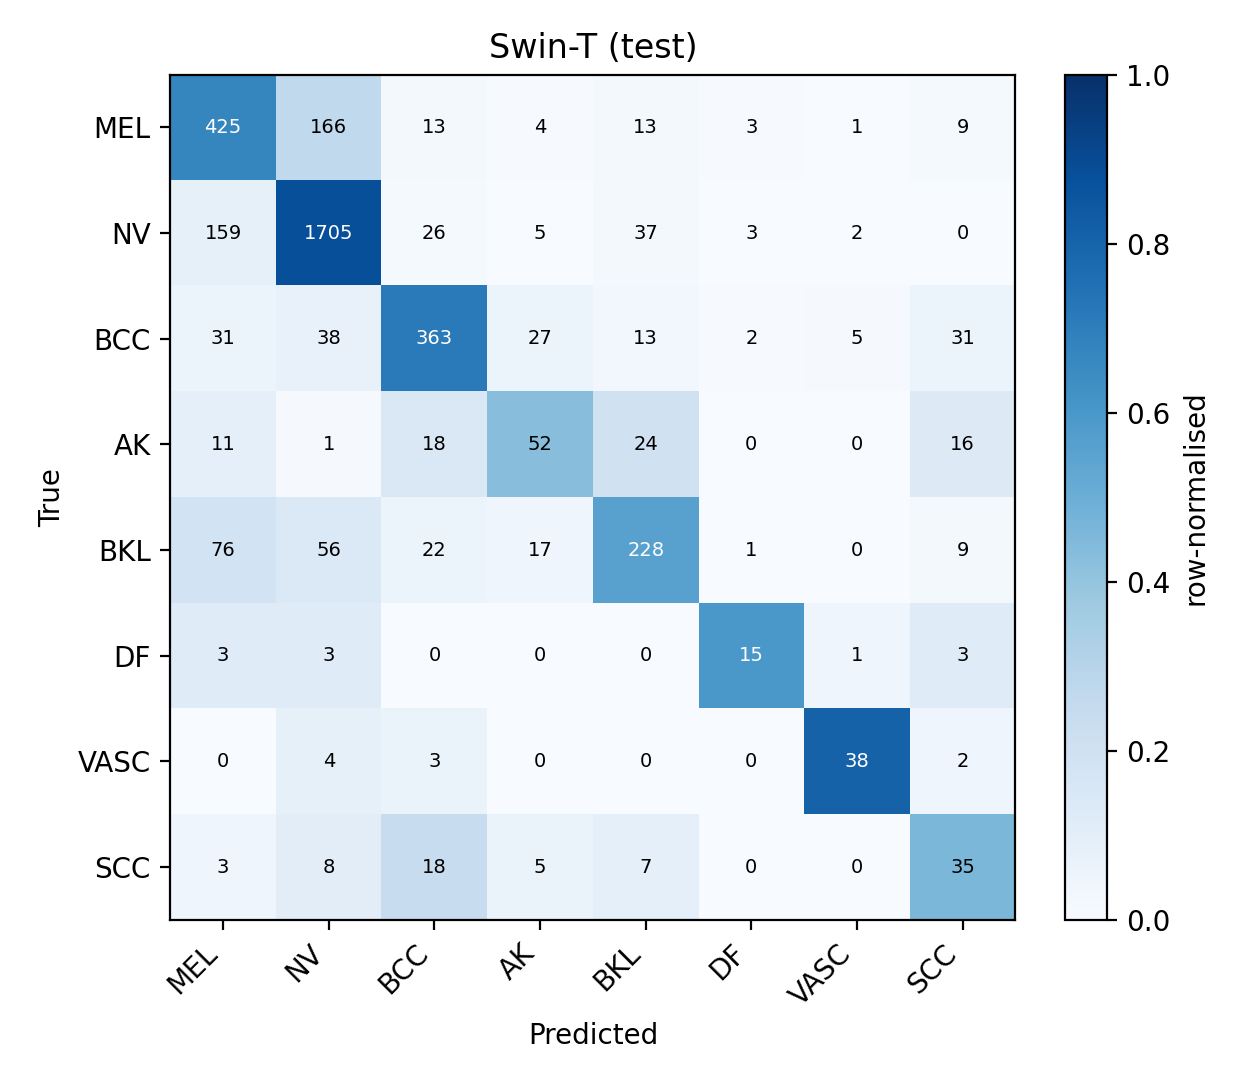
\includegraphics[width=0.32\textwidth]{cm_swin_t.png}
  \caption{Row-normalised confusion matrices on the test split (cell labels are raw counts).}
  \label{fig:cm}
\end{figure*}

\subsection{Interpretability}
Fig.~\ref{fig:gradcam} shows Grad-CAM maps for one test image per class.

\begin{figure}[t]
  \centering
  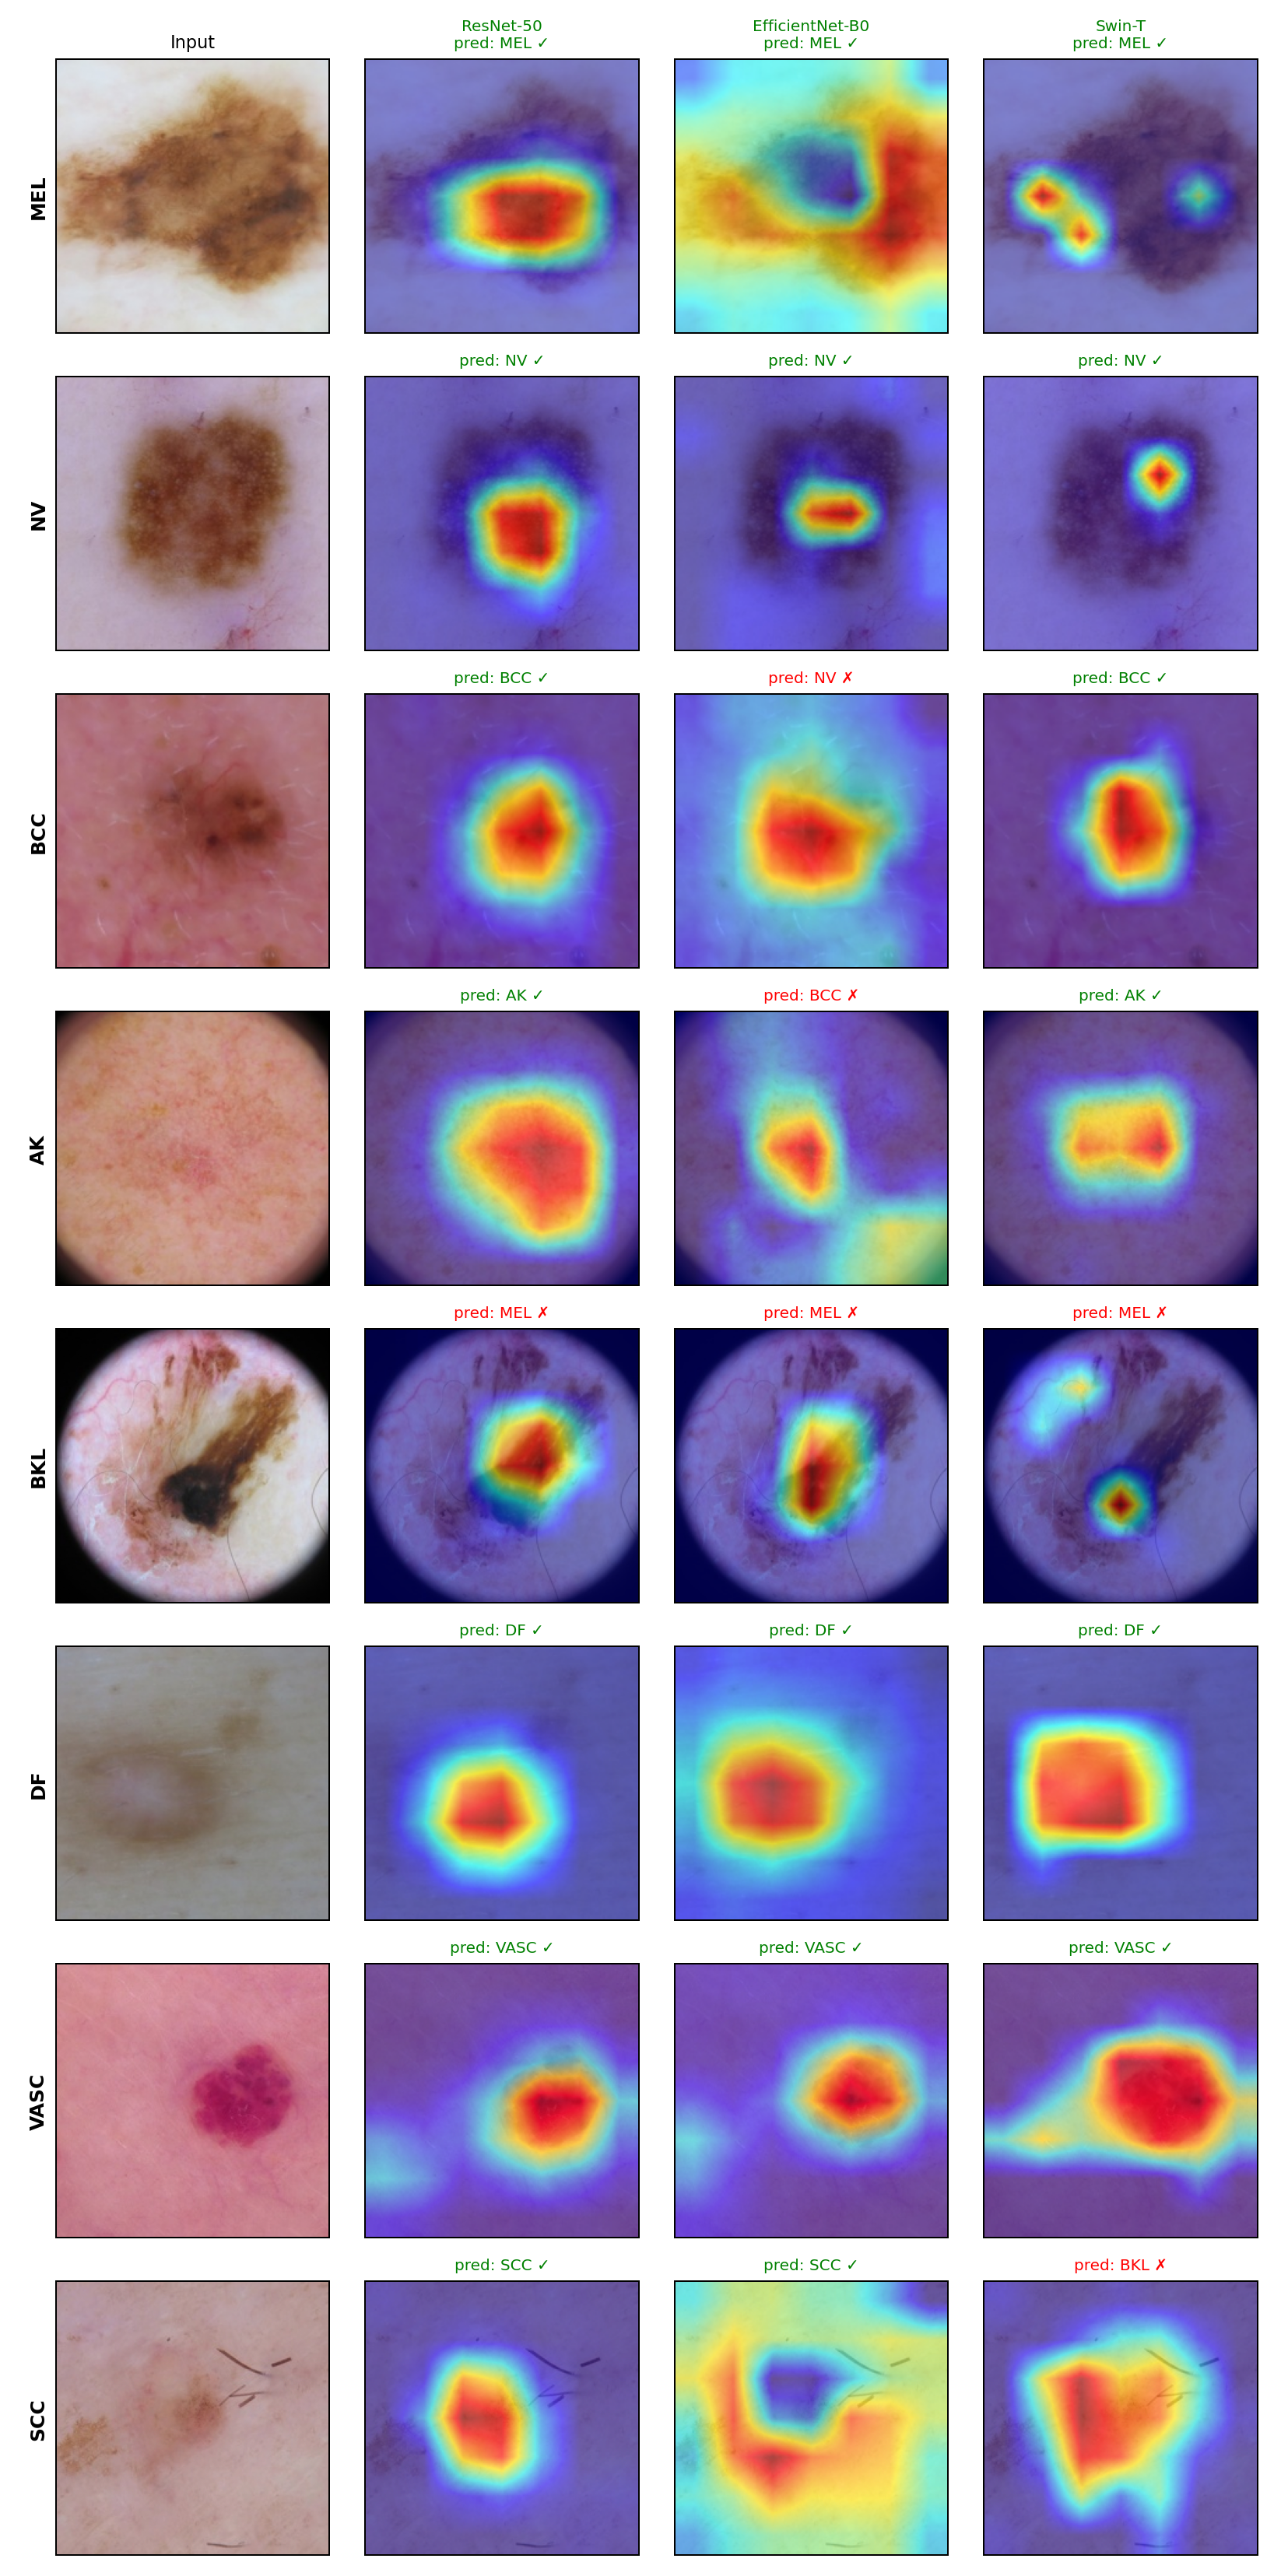
\includegraphics[width=0.96\columnwidth]{gradcam_grid.png}
  \caption{Grad-CAM evidence maps (target = true class) for one test image per class. Green/red
  titles mark correct/incorrect predictions.}
  \label{fig:gradcam}
\end{figure}

\section{Discussion}
\subsection{Which model is ``better''?}
On the decision metrics the ranking is unambiguous: Swin-T is the best single backbone
(\SwinAcc\% accuracy, \SwinBalAcc\% balanced accuracy, \SwinFone\% macro-F1), followed by
EfficientNet-B0 (\EffnetFone\%) and ResNet-50 (\ResnetFone\%). The gap between the transformer and
the best CNN is 6.3 macro-F1 points, which is larger than the 2.7 points separating the two CNNs,
so on this dataset the family label does matter---but not in the direction that is often assumed
for small medical datasets~\cite{matsoukas2021transformers}. Swin-T also converges faster
(\SwinFone\% macro-F1 is already reached at epoch 2 of 12 in validation, Fig.~\ref{fig:curves}),
which we attribute to its stronger ImageNet features and to the hierarchical windowed attention,
which lets it integrate colour and texture cues over the whole lesion rather than within a fixed
receptive field.

The ranking by macro AUC is the \emph{opposite} (ResNet-50 \ResnetAuc{} $>$ EfficientNet-B0
\EffnetAuc{} $>$ Swin-T \SwinAuc{}). AUC measures the quality of the probability ranking of each
class against the rest, whereas accuracy and F1 measure the hard arg-max decision. Swin-T fits the
training set much more tightly (its training loss ends at 1.00 versus 1.42 for ResNet-50 with the
same label smoothing), which produces sharper, more confident posteriors: better decisions on the
hard examples but slightly worse calibrated rankings on the easy ones. This is a reminder that a
single number can hide a trade-off, and that a clinical triage tool that thresholds probabilities
should be evaluated with AUC and calibration, not only with accuracy.

\subsection{Cost: FLOPs are not latency}
EfficientNet-B0 has 6$\times$ fewer parameters and 10$\times$ fewer FLOPs than ResNet-50, trains
in \EffnetTrain{} instead of \ResnetTrain{} minutes and uses the least VRAM
(\EffnetVram{}~GB). Yet on the GPU it is \emph{slower} at inference (\EffnetLat{}~ms versus
\ResnetLat{}~ms at batch~1; \EffnetThr{} versus \ResnetThr{} images/s at batch~32). Its
depthwise-separable convolutions are memory-bound and launch many small kernels that cannot
exploit tensor cores, so the theoretical savings do not materialise on this hardware; they would on
a CPU or mobile NPU, which is the setting EfficientNet was designed for~\cite{tan2019efficientnet}.
Swin-T has almost the same FLOPs as ResNet-50 (\SwinGflops{} versus \ResnetGflops{}~GFLOPs) but is
2.4$\times$ slower at batch~1, needs 1.5$\times$ more VRAM during training
(\SwinVram{} versus \ResnetVram{}~GB) and the longest wall-clock time (\SwinTrain{} min). The
accuracy gain of the transformer therefore has a concrete price: roughly 2.4$\times$ the latency and
1.5$\times$ the training memory of the residual CNN. In a batch setting (offline screening of a
clinic's daily images) this price is negligible; in an interactive or embedded setting it is the
deciding factor.

\subsection{Generalisation across classes}
All models are strong on the majority class NV (F1 0.85--0.88) and on the visually distinctive
VASC and BCC, and weak on the three rare or morphologically overlapping diagnoses AK, SCC and DF
(Table~\ref{tab:perclass}). The confusion matrices (Fig.~\ref{fig:cm}) show two persistent error
clusters: MEL$\leftrightarrow$NV (166 melanomas predicted as nevi and 159 nevi predicted as
melanoma by Swin-T) and the keratinocyte group AK$\leftrightarrow$BKL$\leftrightarrow$SCC, which is
also where dermatologists disagree most. Inverse-square-root class weighting raised the recall of
the rare classes (DF recall 0.60, VASC 0.81, SCC 0.46 for Swin-T) without collapsing the majority
class, but the balanced accuracy of 0.60--0.64 shows that the imbalance is only partly solved.
Swin-T is the most \emph{uniform} model: it has the best F1 in seven of the eight classes and is
the only backbone that lifts DF above 0.6, suggesting that its global receptive field helps on
classes defined by subtle, lesion-wide texture rather than by a local pattern.

\subsection{What the models look at}
The Grad-CAM maps (Fig.~\ref{fig:gradcam}) are consistent with that reading. The two CNNs produce
compact, centred blobs on the pigmented core of the lesion, which is adequate for NV, BCC, DF and
VASC but misses the periphery that distinguishes MEL from NV and AK from BKL. Swin-T produces
sparser, multi-focal maps (e.g. two separated hot spots on the melanoma, a ring on the vascular
lesion) that follow the irregular border and the asymmetric pigment distribution---precisely the
``ABCD'' cues used by clinicians. The failures are informative too: on the BKL example all three
models fire on the darkest region and predict melanoma, and on the SCC example EfficientNet-B0
spreads its evidence over the background, where hair and scale artefacts are present. Such
artefact-driven activations are a known risk on ISIC~\cite{cassidy2022isic} and argue for lesion
segmentation or artefact removal in a deployed system.

\subsection{Are the families complementary?}
The soft-voting ensemble improves on the best single model by 2.3 macro-F1 points
(\EnsFone\% versus \SwinFone\%), by 4.0 balanced-accuracy points and raises the macro AUC to
\EnsAuc{}, the best value in the study. Among the pairwise ensembles, the two CNNs together reach
only 61.5\% macro-F1, whereas EfficientNet-B0+Swin-T reaches 66.4\%, almost the value of the full
ensemble; i.e. nearly all the gain comes from combining a CNN with the transformer. The two
families make different mistakes, which is the strongest practical argument for hybrid systems,
at the cost of \EnsLat{}~ms per image.

\subsection{Comparison with the literature and limitations}
Our balanced accuracies (0.60--0.68) are in the range reported for single ImageNet-pretrained
models on ISIC~2019 at 224~px, and below the 0.63--0.74 obtained by the challenge winner with
multi-resolution EfficientNet ensembles trained on far more compute and with
metadata~\cite{gessert2020isic2019}; note that our numbers are measured on an internal,
in-distribution split and are therefore not directly comparable to the official out-of-distribution
test set. Limitations: a single seed per model (differences below $\approx$1 point should not be
over-interpreted), a fixed 224~px resolution that discards fine dermoscopic structure, no use of
age/sex/site metadata, no test-time augmentation, and a learning rate that was not tuned per
architecture (a per-model search would most likely narrow, not widen, the gaps).


\section{Conclusions and Future Work}
We compared a residual CNN, an efficiency-oriented CNN and a hierarchical vision transformer on
ISIC~2019 under a strictly shared, lesion-grouped protocol and measured accuracy, cost and
interpretability side by side. Three conclusions follow. (i)~With ImageNet pre-training, the
transformer is the most accurate and the most class-uniform backbone on 25k dermoscopic images
(\SwinFone\% macro-F1, \SwinBalAcc\% balanced accuracy), contradicting the view that transformers
need very large medical datasets; its evidence maps also align better with clinical ABCD cues.
(ii)~That accuracy costs about 2.4$\times$ the inference latency and 1.5$\times$ the training memory
of ResNet-50, and the cheapest model by FLOPs (EfficientNet-B0) is not the fastest on a GPU, so
deployment decisions must be based on measured latency on the target hardware rather than on
parameter counts. (iii)~CNNs and transformers make complementary errors: a simple soft-voting
ensemble gives the best macro-F1 (\EnsFone\%) and AUC (\EnsAuc{}) of the study. Our practical
recommendation is EfficientNet-B0 for CPU/edge budgets, Swin-T when a GPU is available, and the
CNN+transformer ensemble for offline screening where accuracy dominates.

Future work should (a)~repeat the study with several seeds and at 384--512~px, where fine
dermoscopic structures become visible; (b)~add patient metadata and test-time augmentation, both
of which helped the challenge winners~\cite{gessert2020isic2019}; (c)~evaluate calibration and
decision thresholds for triage, given the AUC/F1 disagreement observed here; (d)~replace ImageNet
with dermoscopy-specific self-supervised pre-training (DINO/MAE on unlabelled ISIC archives), which
targets the domain gap directly; and (e)~validate externally on the official ISIC~2019 test set
and on clinical (non-dermoscopic) datasets such as PAD-UFES-20 to measure true generalisation.


\section*{Reproducibility}
Code, split file, training logs and all figures are available in the project repository
(\texttt{src/}, \texttt{results/}); \texttt{run\_all.ps1} regenerates every number in this paper
from the public ISIC~2019 download.

\bibliographystyle{IEEEtran}
\bibliography{refs}

\end{document}
